\documentclass[tikz]{standalone}
\usepackage{pgfplots}
\usetikzlibrary{calc}
\begin{document}
    
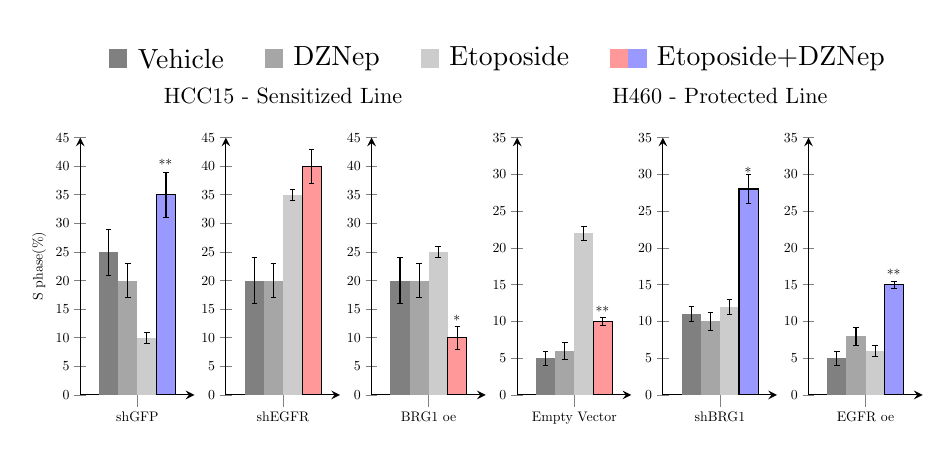
\begin{tikzpicture}
\pgfplotsset{my error bar/.style={error bars/.cd,y dir =both, y explicit}}
\pgfplotsset{
    subplotStyle/.style n args ={1}{
        axis x line = bottom, % change the default axis box.
        axis y line = left,
        width = 0.25\linewidth ,
        height = 0.4\linewidth ,
        ybar=0,
        bar width = 0.02\linewidth ,
        ytick={0,5,...,45},
        ymin=0,ymax=45,
        nodes={scale=0.5},
        xtick=data,
    }
}
\newcommand{\subplotxoffset}{0.4cm}
% plot1 ---------------------------
\newcommand{\subplotName}{shGFP}
\begin{axis}[
    name=plot1,
    ylabel=S phase(\%),
    symbolic x coords={\subplotName},
    subplotStyle={45},
]

\addplot [draw=none,fill=gray!100,my error bar] coordinates {(\subplotName,25)+-(0,4)};
\addplot [draw=none,fill=gray!70,my error bar] coordinates {(\subplotName,20)+-(0,3)};
\addplot [draw=none,fill=gray!40,my error bar] coordinates {(\subplotName,10)+-(0,1)};
\addplot [
    nodes near coords={**},
    nodes near coords style = {
       yshift=15pt,xshift=10pt,
    },
    fill=blue!40,
    my error bar,
    ] coordinates {(\subplotName,35)+-(0,4)};
\end{axis}

% plot2 ----------------------------
\renewcommand{\subplotName}{shEGFR}
\begin{axis}[
    name=plot2,
    at = {($(plot1.east)+(\subplotxoffset,0)$)},
    anchor=west,
    %enlargelimits=0.05,
    symbolic x coords={\subplotName},
    subplotStyle={45},
]
\addplot [draw=none,fill=gray!100,my error bar] coordinates {(\subplotName,20)+-(0,4)};
\addplot [draw=none,fill=gray!70,my error bar] coordinates {(\subplotName,20)+-(0,3)};
\addplot [draw=none,fill=gray!40,my error bar] coordinates {(\subplotName,35)+-(0,1)};
\addplot [fill=red!40,my error bar] coordinates {(\subplotName,40)+-(0,3)};
\end{axis}

% plot3 --------------------------------
\renewcommand{\subplotName}{BRG1 oe}
\begin{axis}[
    name=plot3,
    at = {($(plot2.east)+(\subplotxoffset,0)$)},
    anchor=west,
    %enlargelimits=0.05,
    symbolic x coords={\subplotName},
    subplotStyle={45},
]
\addplot [draw=none,fill=gray!100,my error bar] coordinates {(\subplotName,20)+-(0,4)};
\addplot [draw=none,fill=gray!70,my error bar] coordinates {(\subplotName,20)+-(0,3)};
\addplot [draw=none,fill=gray!40,my error bar] coordinates {(\subplotName,25)+-(0,1)};
\addplot [
    nodes near coords={*},
    nodes near coords style = {
       yshift=5pt,xshift=10pt,
    },
    fill=red!40,my error bar
    ] coordinates {(\subplotName,10)+-(0,2)};
\end{axis}

\renewcommand{\subplotName}{Empty Vector}
\begin{axis}[
    name=plot4,
    at = {($(plot3.east)+(\subplotxoffset,0)$)},
    anchor=west,
    %enlargelimits=0.05,
    symbolic x coords={\subplotName},
    subplotStyle={45},
    ymax=35,
]
\addplot [draw=none,fill=gray!100,my error bar] coordinates {(\subplotName,5)+-(0,1)};
\addplot [draw=none,fill=gray!70,my error bar] coordinates {(\subplotName,6)+-(0,1.2)};
\addplot [draw=none,fill=gray!40,my error bar] coordinates {(\subplotName,22)+-(0,1)};
\addplot [
    nodes near coords={**},
    nodes near coords style = {
       yshift=0pt,xshift=10pt,
    },
    fill=red!40,my error bar] 
    coordinates {(\subplotName,10)+-(0,0.5)};
\end{axis}

% plot5 -----------------------------------
\renewcommand{\subplotName}{shBRG1}
\begin{axis}[
    name=plot5,
    at = {($(plot4.east)+(\subplotxoffset,0)$)},
    anchor=west,
    %enlargelimits=0.05,
    symbolic x coords={\subplotName},
    subplotStyle={45},
    ymax=35,
]
\addplot [draw=none,fill=gray!100,my error bar] coordinates {(\subplotName,11)+-(0,1)};
\addplot [draw=none,fill=gray!70,my error bar] coordinates {(\subplotName,10)+-(0,1.2)};
\addplot [draw=none,fill=gray!40,my error bar] coordinates {(\subplotName,12)+-(0,1)};
\addplot [
    nodes near coords={*},
    nodes near coords style = {
       yshift=5pt,xshift=10pt,
    },
    fill=blue!40,my error bar
    ] coordinates {(\subplotName,28)+-(0,2)};
\end{axis}

% plot6 -----------------------------------
\renewcommand{\subplotName}{EGFR oe}
\begin{axis}[
    name=plot6,
    at = {($(plot5.east)+(\subplotxoffset,0)$)},
    anchor=west,
    %enlargelimits=0.05,
    symbolic x coords={\subplotName},
    subplotStyle={45},
    ymax=35,
    %% the legends to be placed outside 
    legend image code/.code={
        \draw [#1] (0cm,-0.1cm) rectangle (0.2cm,0.1cm);
    },
    legend style={
        legend columns=-1,
        draw=none,
        fill=none,
    },
    legend entries={Vehicle,DZNep,Etoposide,Etoposide+DZNep},
    legend to name=commonLegendb,
]
\addplot [draw=none,fill=gray!100,my error bar] coordinates {(\subplotName,5)+-(0,1)};
\addplot [draw=none,fill=gray!70,my error bar] coordinates {(\subplotName,8)+-(0,1.2)};
\addplot [draw=none,fill=gray!40,my error bar] coordinates {(\subplotName,6)+-(0,0.8)};
\addplot [
    nodes near coords={**},
    nodes near coords style = {
       yshift=0pt,xshift=10pt,
    },
    fill=blue!40,my error bar
    ] 
    coordinates {(\subplotName,15)+-(0,0.5)};
\end{axis}
%% end of the plots ----------------------

% plot the title for the two groups
\node [scale=0.8] (title1) at ($(plot1.north)!0.5!(plot3.north)+(0,15pt)$) {HCC15 - Sensitized Line};
\node [scale=0.8] (title2) at ($(plot4.north)!0.5!(plot6.north)+(0,15pt)$) {H460 - Protected Line};

% self draw the legend ---------------
\node [matrix,fill=none,draw=none] (mylegendnode) at ($(title1.north)!0.5!(title2.north)+(0,8pt)$)
{
\node [fill=gray!100,shape=rectangle,label=right:Vehicle]{}; &[4mm]
\node [fill=gray!70,shape=rectangle,label=right:DZNep]{}; &[4mm]
\node [fill=gray!40,shape=rectangle,label=right:Etoposide]{}; &[4mm]
\node [fill=red!40,shape=rectangle]{}; &
\node [fill=blue!40,shape=rectangle,label=right:Etoposide+DZNep]{}; \\
};

% draw legend with pgfplot function (Not work well)--------------
%\node [scale=0.8] (mylegendnode) at ($(title1.north)!0.5!(title2.north)+(0,8pt)$) {\pgfplotslegendfromname{commonLegendb}};

\end{tikzpicture}

\end{document}